\section{Glossary}
\label{app:glossary}
\begin{description}[leftmargin=1.2em,style=nextline]
\item[pend, r$N$] the model at the end of pretraining; after $N$ rounds of expert iteration.
\item[plain read / guided read] $k=256$ independent attempts per theorem at $T=0.8$ / the same with logically rejected
steps redrawn (at most 10 per attempt). x0, x1: two sample seeds of a plain read.
\item[\sig, \sigp, lemma route] \texttt{DN} on a line built by $\neg$-introduction / \texttt{DN} on any derived line /
proving $\neg\neg G\to G$ inside an implication box and applying it.
\item[free positive reductio] \texttt{DN} on a derived line whose conclusion $G$ is not a negation and whose
$\neg\neg G$ is not a subformula of the theorem, by any route.
\item[strict member] a family member that is classical-only (no intuitionistic proof, by G4ip) and has no $\neg\neg$
subformula in its sequent.
\item[at the bar] a family with at least 50\% of its strict held-out members solved in a plain read.
\item[within reach at $K$] the base's empirical success rate $\hat p \geq 1/K$ over at least $K$ attempts.
\item[certified out of reach at $K$] one-sided 95\% Clopper--Pearson upper bound $< 0.05/K$.
\item[\dcov] theorems RL solves at $k=256$ minus theorems the base reaches within $K$.
\end{description}

\section{Construction of the knockout set}
\label{app:k12ko}
\KTko{} removes every \KT{} record whose written or pruned proof applies \texttt{DN} to a derived double negation
(16,961 records: 16,703 \sig{} and 258 whose \texttt{DN} cites an $\to$-elimination, $\lor$-elimination,
$\bot$-elimination, \texttt{DN} or $\land$-elimination line). It refills 16,961 records, drawn uniformly per length from
\KT{}'s own unused source pools: lengths up to 6 from the depth-3 generator pool and lengths 7--12 from the long-proof
pool. Every refill record passes every \KT{} filter (no box depth $\geq 3$; \texttt{DN} only on assumptions or
premises) and is \sigp-free and lemma-route-free. Under an order-sensitive and a premise-order-invariant renaming key,
the refill shares no class with \KT{} or with any of the 100 data and target files of the repository. One of \KT{}'s 11
exclusion pools was absent when the set was built and could not be checked. Every refill record's proof, translated to
Lean, is accepted (16,961/16,961). Unchanged proofs pass the same harness, and goal-negated proofs fail it. Removal and
refill leave the per-length counts identical. The dose set \KTdose{} swaps 1,550 refill records for removed \sig{}
records at \KT{}'s \sig{} length mix. A 0.1\% set is built but unused.

\section{When each ladder first trained on each family}
\label{app:shares}
First round in which at least half of a family's strict training targets had an accepted proof in the ladder (every
target receives 32 attempts per round; ``--'' = not within 16 rounds).
\begin{center}\small
\begin{tabular}{lcccccc}
\toprule
ladder & contrap.\ conv. & neg.\ cond. & Peirce & Peirce seq. & excl.\ middle & De Morgan \\
\midrule
\Kfull{} s0/s1/s2 & 1/2/1 & 4/13/3 & --/--/3 & --/--/5 & --/14/-- & never \\
\Kfull{} s3/s4/s5 & 2/1/1 & 2/--/-- & 8/--/-- & 3/--/16 & never & never \\
\Kko{} s0--s5 & never & never & never & never & never & never \\
\Kdose{} s0/s1/s2 & 2/1/3 & 3/7/7 & 12/--/-- & 7/--/-- & never & never \\
\bottomrule
\end{tabular}
\end{center}

\section{Budgets at r16 and the estimator}
\label{app:budgets}
At r16 the five allocations are $\Katt = 7{,}147$; $\Ktrain = 17{,}531/15{,}884/20{,}422$; $\Kuni =
24{,}619/22{,}827/29{,}510$; $\Kpub = 47{,}962/49{,}428/50{,}447$; $\Kadapt = 109{,}875/100{,}929/119{,}575$ base
attempts per theorem. Because $\Kadapt$ exceeds the 66,304 attempts most hard theorems received, the r16 sets at
$\Kadapt$ are mostly undetermined. Figure~\ref{fig:estimator} shows the known-proof estimator's calibration.

\begin{figure}[h]
\centering
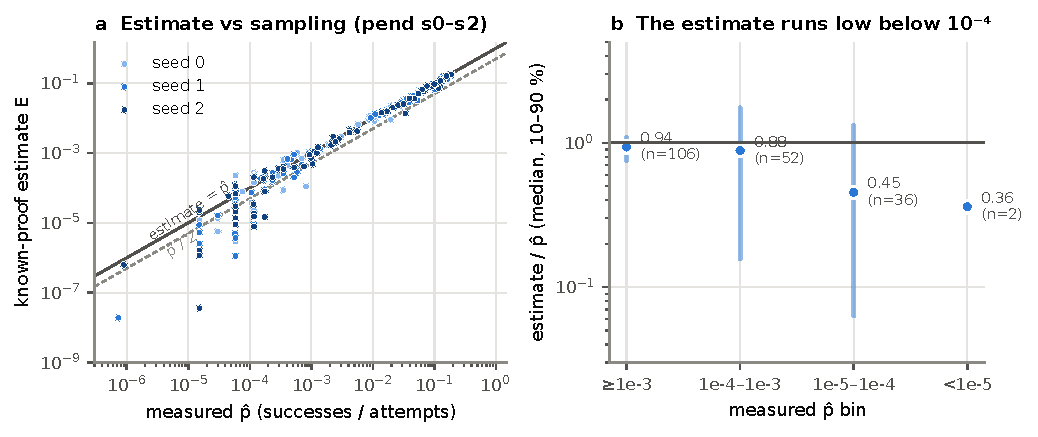
\includegraphics[width=0.92\linewidth]{figures/fig5_estimator.pdf}
\caption{Known-proof estimator, full-exposure bases s0--s2. (a) Estimate against measured $\hat p$ for (seed, theorem)
pairs with at least one success in large-$k$ sampling. (b) Median and 10--90\% range of $E/\hat p$ by $\hat p$ bin.}
\label{fig:estimator}
\end{figure}

\section{Power sampling}
\label{app:power}
The sampler targets $p^\alpha$ over whole proofs by Metropolis--Hastings with suffix resampling
(\texttt{coe/power\_sample.py}): 32 chains per theorem, blocks of 4 proof steps, 8 MH steps per block (32 in the
convergence check), $\alpha \in \{4, 2\}$ (and 1.5 in the control). Acceptance rates were 0.55--0.74. On a development
pilot the per-chain success was 0.752 at 8 MH steps per block and 0.760 at 32. The plain comparators received exactly
the decoded tokens of the power runs. They store no proof text, so their 1--2 solves could not be re-checked in Lean.

\section{Pre-registered expectations against outcomes}
\label{app:expectations}
The experiment's pre-registration stated numeric expectations. As tallied by the reviewer, they \emph{hit} on:
\begin{itemize}
\item the shape of \KTko{};
\item the general-ability gap on held-out greedy decoding and on non-\sig{} theorems;
\item 0/123 strict targets in round 1 and 0/106 held-out members at pend on all knockout seeds;
\item knockout median log-probabilities at or below $-15$ nats;
\item converse contraposition acquired on 3/3 new full seeds;
\item at least one family on 6/6 full and 0/6 knockout seeds;
\item the primary $p$ and the arm medians;
\item recovery of non-classical holdout250 by r16;
\item $\dcov > 0$;
\item the power-sampling nulls;
\item the dose arm's round-1 \sig{} proofs and family acquisition;
\item knockout seed 1's extension.
\end{itemize}
They \emph{missed} on:
\begin{itemize}
\item the classical-only share falling by $\geq 70\%$ (observed 67.6\%);
\item textbook72 within $\pm4$ (observed $-6.5$);
\item certificates on $\geq 5/6$ knockout bases (observed 2/6);
\item negated conditional on $\geq 2/3$ new full seeds (observed 1/3);
\item the first \sigp{} proof after round 4 (it appeared in round 1, on theorems supplying $\neg\neg G$);
\item $\dcov$ within $+8$ to $+35$ (two seeds at $+36$ and $+37$);
\item 0/106 for every sampler on the knockout bases (plain sampling at $T=1$ solved one);
\item 3--15 strict targets in the dose arm's round 1 (observed 2/17/2);
\item a seeded-round gain on $\geq 3$ seeds (observed 1/5).
\end{itemize}

\section{Corrections applied}
\label{app:corrections}
The experiment's own scripts passed two-by-two tables to \texttt{scipy.stats.boschloo\_exact} with the groups as rows.
That function treats columns as groups. With the arms as columns, the RL-only test is $p = 0.0032$ (reported 0.0020),
the excluded-middle test $0.39$ (0.30) and the three-versus-none family tests $0.034$ (0.035). The primary
$p = 0.00024$ and the dose test $p = 0.0033$ are unchanged. \texttt{paper/scripts/stats\_extra.py} recomputes all
five. The reviewer's ten rewordings are applied throughout. The most important ones: ``need'' becomes ``not acquired by
this EI within 16 rounds'', ``reach'' is used only in its technical sense, and the sharpening null is stated for one
sampler.

\section{This paper's checks}
\label{sec:checks}
\emph{[Pending: the pre-registered checks C1--C3 are running; results will be filled in here.]}


\section{Provenance of earlier results}
\label{app:provenance}
Run names refer to reviewed reports in the fork \texttt{dan-pandori/nd-takehome} (branch \texttt{dan\_<run>}, file
\texttt{review\_<run>.md}) and to their summaries in \texttt{nd-rl/experiment-summaries}.
\begin{itemize}
\item \run{create-or-elicit}: the knockout, dose and full s3--s5 ladders; Phase 0 (budgets, estimator) and Phase 2
(power sampling). Review commits \texttt{dd8ee82e} (blind recount), \texttt{8e195390} (verdict).
\item \run{capability-defs}: the measurement framework on full seeds s0--s2 (budgets, certificates, controls,
definitions, guided reads). Review \texttt{da11be78}.
\item \run{trajectory}, \run{rl-continue}: full seeds s0--s2, rounds 1--8 and 9--16; exact likelihoods along RL.
\item \run{rl-from-ckpt}: the replay-only control.
\item \run{guided-tts}: guided redraws at matched tokens; the step checker.
\item \run{mcts-a}: PUCT search with a learned value (review \texttt{5e70afbd}).
\item \run{grpo-best}: GRPO variants from the same checkpoints.
\item \run{support-curves}, \run{support-state}, \run{claim-audit}: the 3.2M organism and the interface confound.
\end{itemize}
The claims ledger (\texttt{claims\_ledger.md}, rows L1--L101) maps every inherited number to its reviewed source.
